\documentclass[12pt]{exam}
\usepackage{amsthm}
\usepackage{libertine}
\usepackage[utf8]{inputenc}
\usepackage[margin=0.7in]{geometry}
\usepackage{amsmath,amssymb}
\usepackage{multicol}
\usepackage[shortlabels]{enumitem}
\usepackage{siunitx}
\usepackage{cancel}
\usepackage{marvosym}
\usepackage{graphicx}
\usepackage{pgfplots}
\usepackage{xcolor}
\usepackage{listings}
\usepackage{amsmath}
\usepackage{tikz}
\usepackage{booktabs}
\usepackage{hyperref}
\usepackage{subcaption}
\usepackage{titling}
\usepackage[T1]{fontenc}
\usepackage{underscore}
\usepackage{algorithm2e}
\usepackage{pdfpages}


\let\head\relax
\let\foot\relax
\let\cfoot\relax
\let\chead\relax
\let\lfoot\relax
\let\lhead\relax
\let\rfoot\relax
\let\rhead\relax
\usepackage{fancyhdr}

\usepackage{lipsum} 
\usepackage{url}
\urlstyle{sf}
\renewcommand\UrlFont{\color{blue}\sffamily}
\pgfplotsset{width=10cm,compat=1.9}
\usepgfplotslibrary{external}
\tikzexternalize
\newcommand{\class}{AI5213/EC4213: Machine Learning and Deep Learning} 
\newcommand{\examnum}{Homework 3 (Kaggle Competition)} 
\newcommand{\timelimit}{}
\renewcommand{\headrulewidth}{0pt}

\definecolor{pastelyellow}{RGB}{255, 255, 224}
\definecolor{lightorange}{RGB}{255, 200, 150}

\lstdefinestyle{mystyle}{
    backgroundcolor=\color{pastelyellow},  
    commentstyle=\color{olive},
    keywordstyle=\color{blue},
    % numberstyle=\tiny\color{gray},
    % numbers=left,
    % numbersep=5pt,
    % showspaces=false,
    % showstringspaces=false,
    % showtabs=false,
    % tabsize=2,
    % breaklines=true,
    % breakatwhitespace=true,
    % title=\lstname,
    basicstyle=\sffamily\small,
    frame=single,
    rulecolor=\color{lightorange}, 
}

\lstdefinestyle{inlinecode}{
  basicstyle=\ttfamily\small,
  breaklines=true,
  backgroundcolor=\color{lightgray},
  language=python,
  showstringspaces=true
}

\lstset{style=mystyle}

\fancypagestyle{firststyle}
{
   \fancyfoot[C]{\footnotesize{GIST AI5213/EC4213/AI4021/CT5303/ET5402/FE5402, Fall 2025, Instructor: Sundong Kim.}} 
}
% }

\title{\vspace{-2em}\sffamily\bfseries
  Used-Car Price Prediction
  \vspace{-0.7em}
}
\author{\sffamily
  \textit{Kaggle GIST-MLDL-25F-HW3 Competition}\\[0.3em]
  \\
  Jumyung Park    \textit{\#20235073}\\
  \small School of EECS, Gwangju Institute of Science and Technology\\[0.2em]
}
\date{}


\begin{document}
\thispagestyle{firststyle}

\noindent
\begin{tabular*}{\textwidth}{l @{\extracolsep{\fill}} r @{\extracolsep{6pt}} l}
  \textbf{\class} & \textbf{Student ID:} &  20235073 \\

  \textbf{\examnum}  & \textbf{\lstinline[style=inlinecode]|Name|:} &  Jumyung Park \\
\end{tabular*}\\
% {
\noindent \rule[1ex]{\textwidth}{1pt}
% ---

\noindent{\textbf{Due: Sunday, Nov 16, 11:59PM}}


\hspace{1mm}

\noindent Welcome to HW3! This assignment features a Kaggle competition on car price prediction, where you'll engineer effective features and apply the machine learning models. The homework consists of a prediction competition and a technical report.

\vspace{2mm}
{\centering
  \fbox{\centering \begin{minipage}{.95\textwidth}

      \textbf{Essential Resources:}
      \begin{itemize}[itemsep=0cm]  % Reduced from default spacing
        \item Tree Models in ISLP: \url{https://islp.readthedocs.io/en/latest/labs/Ch08-baggboost-lab.html}
        \item Kaggle Competition Guide: \url{https://www.kaggle.com/learn/guide/kaggle-competitions}
        \item Feature Engineering: \url{https://www.kaggle.com/learn/feature-engineering}
      \end{itemize}
      \textbf{Recommended Workflow:}
      \begin{itemize}[itemsep=0cm]  % Reduced from default spacing
        \item Start with EDA and basic data cleaning
        \item Implement a baseline model (e.g., decision tree, GAM) and get used to submitting your results
        \item Gradually explore advanced models (Random Forest, XGBoost) and ensemble them
        \item Use cross-validation to prevent overfitting
        \item Document your progress and insights
      \end{itemize}

    \end{minipage}}}

\vspace{5mm}
\noindent \textbf{Deliverables:}
\begin{itemize}[itemsep=0.1cm]  % Reduced from default spacing
  \item Submit a single PDF via Gradescope (``HW3 Write-Up")
  \item Include your competition results and technical report
  \item Attach your code in the appendix
  \item If you use any external dataset for training, please write the link to the dataset.
  \item Use LaTeX template provided (or neat handwriting if necessary)
\end{itemize}

\vspace{3mm}
\noindent \textbf{Important Guidelines:}
\begin{enumerate}[itemsep=0.1cm]  % Reduced from default spacing
  \item Sign the honor code statement on the next page
  \item Document any collaboration or help received
  \item Write all responses in English
  \item Properly mark question sections in Gradescope
\end{enumerate}


\vspace{7mm}

\noindent \textbf{For staff use only} \vspace{-3mm}
\begin{table}[ht]
  \centering
  \setlength{\tabcolsep}{0.35cm}
  \renewcommand{\arraystretch}{1.3}
  \begin{tabular}{r|r|r|r} \toprule
    Q1 (Part 1)      & Q2 (Part 2)      & \phantom{/5} Bonus \phantom{/5} & \phantom{/5} Total \phantom{/5} \\ \midrule
    \phantom{/5}/ 40 & \phantom{/5}/ 50 & \phantom{/5}/ 10                & \phantom{/5}/ 90                \\ \bottomrule
  \end{tabular}
\end{table}
% }
% ------------------------- Honor Code ------------------------------------%

\newpage
\pagestyle{fancy}
\noindent {\large Honor Code }

\vspace{3mm}
\noindent \textbf{Declare and sign the following statement:}

\vspace{3mm}
\noindent \textit{“I certify that all solutions in this document are entirely my own and that I have not looked at
  anyone else’s solution. I have given credit to all external sources I consulted.”}

\vspace{5mm}

\noindent {\large \textit{Signature}}: Jumyung Park

\vspace{5mm}

\noindent We welcome group discussions, but the work you submit should be entirely your own. If you use any information or pictures not from our lectures or readings, make sure to say where they came from. Please note that breaking academic rules can lead to severe penalties.

\begin{enumerate}[label=(\alph*), itemsep=4cm]

  \item Did you receive any help whatsoever from anyone in solving this assignment? If your answer is ‘yes’, give full details (e.g., “Alex shared insights on optimizing hyperparameters for XGBoost during a group discussion.”)

        \fbox{
          \begin{minipage}{38em}
            No
          \end{minipage}
        }

  \item Did you give any help whatsoever to anyone in solving this assignment? If your answer is ‘yes’, give full details (e.g., “I advised Chris to check out the Kaggle feature engineering guide for handling missing values.”)

        \fbox{
          \begin{minipage}{38em}
            No
          \end{minipage}
        }

  \item Did you find or come across code that implements any part of this assignment? If your answer is ‘yes’, give full details (book \& page, URL \& location within the
        page, etc.).

        \fbox{
          \begin{minipage}{38em}
            I followed the feature engineering tutorial on \url{https://www.kaggle.com/learn/feature-engineering}, which was listed in the essential resources.
          \end{minipage}
        }

\end{enumerate}



\newpage
\noindent {\large Q1. Mini Competition: Car \lstinline[style=inlinecode]|Price| Prediction [100 pts] \Keyboard}

\vspace{5mm}
\noindent In this mini-competition, you'll work with real-world data to build and improve your predictive models. Your journey will be evaluated on two aspects: your model's performance on the Kaggle leaderboard (40 points) and a technical report documenting your approach (50 points). Bonus points will be awarded as follows: 5 points for the best reports and 5 points for the best competitors.

\vspace{5mm}
\noindent \textbf{Part 1: Competition Performance [40 pts]}

\vspace{5mm}
\noindent Your task is to predict car prices. Strive to surpass the target score and submit your results. You're free to use any libraries available - such as \textsf{scikit-learn}, \textsf{pandas}, \textsf{numpy}, \textsf{statsmodel}, \textsf{ISLP}, \textsf{xgboost}, \textsf{polars} and others. Your grade for this part will be determined entirely by your final performance on the private leaderboard. Follow these simple rules: Use your student ID, play fair, give it your all, and, most importantly, enjoy the mini-competition: \url{https://www.kaggle.com/t/7fb5c52dc7bee6f4b9eff6a4e40bcd83}

\vspace{5mm}
\textbf{Score guideline}
\begin{itemize}[itemsep=0.2cm]
  \item The leaderboard uses Mean Absolute Percentage Error (MAPE) as the evaluation metric, where smaller scores indicate better models.
  \item While you'll see and capture your public leaderboard score during development, final grading will be based on the private leaderboard score to ensure your model generalizes well to unseen data.
  \item You can submit up to five times per day. We encourage you to divide the dataset into train/validation sets and use your internal validation set to select the best model for submission.
  \item Final points will be determined by your private leaderboard score $s$ with the target score $t$.
  \item Who achieved better than the target score $(s \leq t)$ will receive the full points (40 pts).
  \item Those who didn't beat the target score $(t < s)$ will receive $40 * \min((t/s), 1)$ points.
  \item You're free to use the Ed \& Kaggle discussion tab for sharing your thoughts or your code snippets.
  \item Referencing or reusing code from other students, making multiple accounts will be treated as an honor code violation. (Honor code at \url{https://sundong.kim/courses/mldl25f})
\end{itemize}

\begin{figure}[ht!]
  \centering
  \includegraphics[width=0.7\linewidth]{figures/id.png}
  \caption{Use your student ID as a team \lstinline[style=inlinecode]|Name|}
  \label{fig:enter-label}
\end{figure}



\newpage
\noindent \textbf{Part 2: Technical Report [50 pts]}
\vspace{5mm}

\noindent Write a self-contained report (at most 5 pages) documenting your approach and findings. For reference on how to structure your report, you can check example write-ups at \url{https://wsdm-cup-2018.kkbox.events/}. The report should comprehensively document all stages of your analytical process and methodology.

\vspace{5mm}
\noindent Your report should include:
\begin{itemize}[itemsep=0.2cm]
  \item \textbf{Problem Description and Data}
        \begin{itemize}
          \item Clear statement of the task and evaluation metric
          \item Dataset characteristics and initial insights
          \item Train/validation split strategy
        \end{itemize}
  \item \textbf{Data Preprocessing \& Feature Engineering}
        \begin{itemize}
          \item Data cleaning and handling of missing values/outliers
          \item Feature creation rationale and importance analysis
          \item Feature selection process
        \end{itemize}
  \item \textbf{Modeling \& Results}
        \begin{itemize}
          \item \lstinline[style=inlinecode]|Model| architecture and validation methodology
          \item Hyperparameter tuning strategy
          \item Performance analysis and key findings
        \end{itemize}
  \item \textbf{Technical Implementation}
        \begin{itemize}
          \item Key libraries/frameworks used
          \item Challenges faced and solutions
        \end{itemize}
\end{itemize}

\vspace{2mm}
\noindent \textbf{Format requirements:}
\begin{itemize}[itemsep=0.2cm]
  \item Please limit the main document to 5 pages in the current single-column LaTeX format, with unlimited references allowed beyond the page limit. (Use the template at the end of this document; longer submissions will be penalized significantly)
  \item Include a screenshot of your public leaderboard score as evidence
  \item Include representative code snippets for important steps \\ (Data preprocessing, feature engineering, model training)
  \item Include relevant figures/tables to support your discussion
  \item Proper citations if you reference any external resources
  \item Clear structure with appropriate section headers
  \item Use clear and concise technical writing
\end{itemize}
\newpage
\noindent \textbf{Assessment Guidelines}
\begin{itemize}[itemsep=0.2cm]
  \item \textbf{Data Type Conversion}
        \begin{itemize}
          \item Correctly convert string features to numeric (e.g., ``20.0 kmpl" → 20.0)
          \item Handle multiple units within the same feature
          \item Document your conversion strategy and ensure consistency
        \end{itemize}

  \item \textbf{Missing Values and Outliers}
        \begin{itemize}
          \item Thoroughly check for missing values in all columns
          \item Document your strategy for handling missing data
          \item Document and justify your handling strategy for missing values
          \item Identify and appropriately handle outliers with justification
        \end{itemize}


  \item \textbf{Data Splitting Strategy}
        \begin{itemize}
          \item Explain your choice of split ratio and methodology
        \end{itemize}

  \item \textbf{Feature Engineering}
        \begin{itemize}
          \item Create meaningful derived features based on domain knowledge
          \item Analyze feature importance and select relevant features
          \item Document the rationale behind each engineered feature
        \end{itemize}

  \item \textbf{Model Training and Evaluation Metrics}
        \begin{itemize}
          \item Justify your choice of training objective and explain the relationship between training metric and evaluation metric
          \item Report how you conduct a comprehensive performance assessment on your validation set.
        \end{itemize}

  \item \textbf{Hyperparameter Tuning}
        \begin{itemize}
          \item Manually search for optimal hyperparameters (grid search or random search)
          \item Show iterative improvements through parameter tuning
        \end{itemize}

  \item \textbf{Prohibited Tools/Methods}
        \begin{itemize}
          \item Automated hyperparameter tuning libraries (e.g., Optuna, Hyperopt, Ray Tune)
          \item AutoML frameworks (e.g., Auto-sklearn, TPOT, H2O AutoML, PyCaret's automated comparison)
        \end{itemize}
\end{itemize}

\newpage
\noindent \textbf{Required Evidence of Manual Work:}

\vspace{5mm}
\noindent To demonstrate genuine understanding and ensure academic integrity, your report must include:

\begin{enumerate}[itemsep=0.3cm]

  \item \textbf{Experimental Process and Comparisons}
        \begin{itemize}
          \item Document your iterative development showing progressive improvements
          \item Compare multiple approaches systematically:
                \begin{itemize}
                  \item Different models (e.g., Random Forest vs XGBoost)
                  \item Different preprocessing strategies (outlier handling, target transformation)
                  \item Different strategies for high missing rate features
                \end{itemize}
          \item Present results in comparative tables or visualizations
          \item Hyperparameter Search Documentation
                \begin{itemize}
                  \item Provide a table showing at least 3 different hyperparameter combinations you tested
                  \item Include validation performance for each configuration
                \end{itemize}
        \end{itemize}

        \noindent Example table format:
        \begin{table}[ht]
          \centering
          \small
          \begin{tabular}{|c|c|c|c|c|}
            \hline
            \textbf{Config} & \textbf{n\_estimators} & \textbf{max\_depth} & \textbf{learning\_rate} & \textbf{MAPE} \\
            \hline
            1               & 100                    & 5                   & 0.1                     & 0.38          \\
            2               & 200                    & 5                   & 0.1                     & 0.37          \\
            3               & 200                    & 7                   & 0.1                     & 0.36          \\
            4               & 200                    & 7                   & 0.05                    & 0.25          \\
            5               & 300                    & 7                   & 0.05                    & 0.20          \\
            \hline
          \end{tabular}
          \caption{Example of documented hyperparameter search process}
        \end{table}

  \item \textbf{Feature Engineering Justification}
        \begin{itemize}
          \item For each significant engineered feature:
                \begin{itemize}
                  \item \textit{Motivation:} Why you created it
                  \item \textit{Implementation:} How you computed it (with code)
                  \item \textit{Impact:} Performance change after adding it
                \end{itemize}
          \item Example: ``Created \texttt{booking\_days\_advance} = \texttt{departure\_date} - \texttt{booking\_date} because early bookings are typically cheaper. Correlation: -0.64, improved MAPE from 0.32 to 0.25."
        \end{itemize}

  \item \textbf{Code Transparency}
        \begin{itemize}
          \item Include code snippets for key steps with manual implementation
          \item Comment your code to explain design choices
          \item Avoid showing only high-level library calls without context
        \end{itemize}
\end{enumerate}

\vspace{2mm}
\noindent If you are uncertain whether a specific tool or method is allowed, please consult with staffs before using it.

\newpage
\noindent \textbf{Part 3: Bonus Points [10 pts]}
\vspace{5mm}

\noindent Outstanding submissions that demonstrate exceptional quality and performance can earn up to 5 bonus points.

\vspace{3mm}
\noindent \textbf{Bonus Point Categories:}

\begin{itemize}[itemsep=0.3cm]
  \item \textbf{Exceptional Report Quality [up to 5 pts]}
        \begin{itemize}
          \item Top 10 reports demonstrating exceptional analysis and documentation
          \item Selected based on:
                \begin{itemize}
                  \item Depth and breadth of experimental comparisons
                  \item Quality and clarity of explanations and visualizations
                  \item Insightful analysis of results, including thorough error analysis
                  \item Professional presentation with well-structured narrative
                  \item Evidence of critical thinking and creative problem-solving
                \end{itemize}
        \end{itemize}

  \item \textbf{Outstanding Leaderboard Performance [up to 5 pts]}
        \begin{itemize}
          \item Top 10 submissions on the final private leaderboard (based on MAPE)
          \item Demonstrates effective modeling and feature engineering in practice
        \end{itemize}
\end{itemize}

\vspace{3mm}
\noindent \textbf{Important Notes:}
\begin{itemize}
  \item Students who qualify for both categories (exceptional report and top 10 leaderboard) will receive 10 bonus points in total
  \item Bonus points are awarded at the instructors' and TAs' discretion
  \item Focus on demonstrating thorough understanding and thoughtful experimentation rather than solely pursuing the highest score
  \item Quality of explanation and justification matters as much as final performance
\end{itemize}

\vspace{3mm}
\noindent \textbf{What Makes a Report Exceptional:}

\noindent Reports that stand out typically include:
\begin{itemize}
  \item Multiple well-designed experiments with clear comparisons
  \item Thoughtful handling of challenging aspects (e.g., high missing rate features, outliers, etc..)
  \item Clear documentation of the iterative development process
  \item Professional visualizations that effectively communicate insights
  \item Honest discussion of what worked and what didn't, with analysis of why
  \item Evidence of going beyond minimum requirements with creative approaches
  \item Clear, well-organized writing that tells a coherent story
\end{itemize}

\clearpage

% --------------------------------------------------------------------------------------------

\maketitle{}


\section {Task and Data}

\subsection{Task}
The task of this competition (GIST-MLDL-25F-HW3 \cite{mldl25f-kaggle}) is to predict the price of a used car.
Performance is evaluated with Mean Absolute Percentage Error (MAPE) between the predicted price and actual price.
Training dataset is public while test dataset's target variable is private.
The prediction will be evaluated on MAPE measure on the hidden test dataset target varaible.

\subsection{Dataset}
The dataset consists of features listed in Table \ref{tab:datadescription}.
Total 4470 training samples are provided and test dataset consists of 1491 rows, without the target variable \lstinline[style=inlinecode]|Price|.
Target variable is numerical, thus the task is a regression problem of predicting the numerical value of \lstinline[style=inlinecode]|Price| with all the other features.
Features contain both categorical and numerical values. Some features have missing values and mixed units.
These inconsistencies were addressed in data preprocessing.

\begin{table*}[ht!]
  \centering
  \caption{Data description}
  \label{tab:datadescription}
  \small
  \resizebox{0.8\linewidth}{!}{
    \begin{tabular}{ l | c | l } \toprule
      Feature           & Data Type & Explanation                                                          \\
      \midrule
      ID                & str       & Unique identifier for each car listing                               \\
      Name              & str       & The brand and model Name of the car                                  \\
      Location          & str       & The city where the car is being sold                                 \\
      Year              & int       & Manufacturing year of the vehicle                                    \\
      Kilometers_Driven & int       & Total distance the car has been driven (in kilometers)               \\
      Fuel_Type         & str       & Type of fuel the car uses (Petrol, Diesel, CNG, LPT, Electric)       \\
      Transmission      & str       & Type of transmission system (Manual or Automatic)                    \\
      Owner_Type        & str       & Number of previous owners (First, Second, Third, Forth \& and Above) \\
      Mileage           & str       & Fuel efficiency of the car (kmpl or km/kg)                           \\
      Engine            & str       & Engine displacement in cubic centimeters (CC)                        \\
      Power             & str       & Maximum power output of the engine (bhp - brake horse power)         \\
      Colour            & str       & Exterior color of the vehicle                                        \\
      Seats             & int       & Number of seating capacity                                           \\
      No. of Doors      & int       & Number of doors in the vehicle                                       \\
      New_Price         & str       & Original price of the car when it was new                            \\
      \midrule
      Price             & float     & Target variable: Current selling price of the used car (in lakhs)    \\
      \bottomrule
    \end{tabular}
  }
\end{table*}


\section{Data Preprocessing and Feature Engineering}


\subsection{Data Preprocessing}
The dataset was thoroughly inspected feature by feature to spot any inconsistencies in representations and remedy them so that any further processings down the line does not get unexpected errors.
Multiple issues in representation was found in the process.

\begin{itemize}[itemsep=0pt, parsep=0pt, topsep=5pt, partopsep=0pt]
  \item Missing values denoted with the string \lstinline[style=inlinecode]|\\N| were replaced with \lstinline[style=inlinecode]|None|.
  \item \lstinline[style=inlinecode]|New_Price| was in mixed units (Lakh and Cr). It was parsed and converted to Lakh unit.
  \item \lstinline[style=inlinecode]|Mileage| was in mixed units (kmpl and km/kg). It was parsed and converted to kmpl unit.
  \item \lstinline[style=inlinecode]|Price| and \lstinline[style=inlinecode]|New_Price| had non-negligible amount of missing values (each 2.37\% and 86.31\% of training dataset). This had to be carefully addressed in feature engineering.
  \item For the processing on dataframes on the following processes, each features were converted to `category' or their respective numerical datatypes after standardizing units and parsing.
\end{itemize}

Unit standardization in \lstinline[style=inlinecode]|New_Price| was straight forward since Lakh and Cr were just different scales of the same measure (1 Cr = 100 Lakh).
However, unit standardization in \lstinline[style=inlinecode]|Mileage| were between two different measures.
Liters is a measure of volume and Kg is a measure of mass.
Therefore, \lstinline[style=inlinecode]|Fuel_Type| was used in the conversion to determine the density to use in the convesion.
Fuel density for each fuel type was used in this preprocessing as an external knowledge.
Since \lstinline[style=inlinecode]|Fuel_Type| had no missing values in both training and test dataset, the conversion factor derivation from it was available for all given \lstinline[style=inlinecode]|Mileage| values.
Details in the process is documented in the notebook code attached as Apendix \ref{appendix:preprocessing-nb}

\subsection{Feature Engineering}
\subsubsection{Systematic Feature Engineering Process}
Given the preprocessed data, feature engineering was performed systematically to remove noise and extract information as much as possible.
The purpose of this systematic process was to not miss any processings that can be done and make data-driven decisions on whether to adopt or discard the attempted engineering.
It is essentialy a manual greedy forward selection with cross validation.
This systematic approach turned out to be effective in building the optimal pipeline while trying numerous approaches in scale, which led to 0.12191 MAPE score on public leaderboard without any tuning on the model.
In fact, around 30 transformations were attempted and 13 of them were adopted to form the final feature engineering pipeline. Some of the non-trivial feature engineerings are highlighted in the following subsections. The entire feature-engineering process is documented in the notebook in Appendix \ref{appendix:feature-engineering-nb}.


\subsubsection{Feature-by-Feature Engineering}
\paragraph{
  Name Splitting and Target Encoding
}
\lstinline[style=inlinecode]|Name| is string feature consisting of \lstinline[style=inlinecode]|Brand| and \lstinline[style=inlinecode]|Model|.
Since \lstinline[style=inlinecode]|Name| has large cardinality, it was split into \lstinline[style=inlinecode]|Brand| and \lstinline[style=inlinecode]|Model|.
For robustness, an enum of recognized brands was constructed and used for extracting \lstinline[style=inlinecode]|Brand| and \lstinline[style=inlinecode]|Model| from \lstinline[style=inlinecode]|Name|.
Since \lstinline[style=inlinecode]|Brand| and \lstinline[style=inlinecode]|Model| have a hierarchical relationship, various methods including dropping \lstinline[style=inlinecode]|Model|, dropping \lstinline[style=inlinecode]|Name|, target encoding \lstinline[style=inlinecode]|Model|, \lstinline[style=inlinecode]|Brand|, or \lstinline[style=inlinecode]|Name|, or all of them were attempted.
Among those, including and target encoidng \lstinline[style=inlinecode]|Model|, \lstinline[style=inlinecode]|Brand|, and \lstinline[style=inlinecode]|Name| yielded the biggest gain compared to the estabished baseline with only preprocessing.
Exploiting the hierarchical relationship, creating \lstinline[style=inlinecode]|Model_Preimum| feature to represent tier within the \lstinline[style=inlinecode]|Brand| was attempted, but discarded due to no visible gain of performance.
Engineering on \lstinline[style=inlinecode]|Name| turned out to be one of the most critical process, resulting in -0.0101 reduction in cv-score compared to the baseline.

\paragraph{Power Imputation}
\lstinline[style=inlinecode]|Power| feature had non-negligible amount of missing values (2.37\% of training data, and 1.95\% of test data).
Utilizing the domain knwoledge that the engine displacement is directly related to its power in combustion, I inspected its correlation with \lstinline[style=inlinecode]|Engine| and it showed high correlation of 0.86.
Exploiting this correlation, PowerImputer was constructed by fitting a linear regression on \lstinline[style=inlinecode]|Power| to \lstinline[style=inlinecode]|Engine| and using it to interpolate the missing \lstinline[style=inlinecode]|Power| value.
Fortunately, there were dense enough samples around the missing \lstinline[style=inlinecode]|Power| values and thus could be faithfully inferred.
This imputation led to 0.0055 reduction in MAPE score, compared to the baseline without any feature engineering.

\begin{figure*}[ht!]
  \centering
  \includegraphics[width=0.5\linewidth]{figures/impute-power.png}
  \caption{Imputation of \lstinline[style=inlinecode]|Power| using its correlation to \lstinline[style=inlinecode]|Engine|}
  \label{fig:imput-power}
\end{figure*}

\paragraph{Non-Linear Transformation on Price}
The target feature \lstinline[style=inlinecode]|Price| was heavily skewed.
Applying logarithmic transformation relieved the skewness and led to 0.0150 drop of MAPE cross validation score, which indicate that the transformation was very effective.

\begin{figure*}[ht!]
  \centering
  \begin{subfigure}[b]{.4\linewidth}
    \centering\captionsetup{width=\linewidth}%
    \includegraphics[width=\linewidth]{figures/price-before-transformation.png}
    \caption{\lstinline[style=inlinecode]|Price| distribution before transformation}
  \end{subfigure}
  \begin{subfigure}[b]{.4\linewidth}
    \centering\captionsetup{width=\linewidth}%
    \includegraphics[width=\linewidth]{figures/price-after-transformation.png}
    \caption{\lstinline[style=inlinecode]|Price| distribution after transformation}
  \end{subfigure}
  \caption{\lstinline[style=inlinecode]|Price| distribution of before and after logarithmic transformation}
  \label{fig:price-transformation}
\end{figure*}

\paragraph{
  Adopted Pipeline
}
As a result of feature-by-feature engineering, the adopted pipeline consisted of extracting \lstinline[style=inlinecode]|Brand| and \lstinline[style=inlinecode]|Model|, target-encoding \lstinline[style=inlinecode]|Brand|, \lstinline[style=inlinecode]|Model|, and \lstinline[style=inlinecode]|Name|, transforming \lstinline[style=inlinecode]|Year| to \lstinline[style=inlinecode]|Age|, clipping unrealistic \lstinline[style=inlinecode]|Kilometers_Driven|, grouping rare \lstinline[style=inlinecode]|Fuel_Type|, clipping unrealistic \lstinline[style=inlinecode]|Mileage|, imputing power by predicting with \lstinline[style=inlinecode]|Fuel_Type|, binning \lstinline[style=inlinecode]|Seats|, log transforming \lstinline[style=inlinecode]|Price|, category encoding, and log transforming \lstinline[style=inlinecode]|Price|.
Evaluated with cross-validation, MAPE score decreased by 0.0229 compared to the baseline, which is a significant gain of performance.
Details of this pipeline is included in the Table \ref{tab:feature-engineering-pipeline}

\subsubsection{Interaction Features}
Building on top of independently engineered features, several interaction features were attemped.

\paragraph{Data-Driven Approach}
By calculating the correlation plot on the residuals of the model predictions, \lstinline[style=inlinecode]|Engine|, \lstinline[style=inlinecode]|Price|, \lstinline[style=inlinecode]|Power|, \lstinline[style=inlinecode]|Brand|, \lstinline[style=inlinecode]|Model|, and \lstinline[style=inlinecode]|Name| was found to have high correlation in the residuals.
Starting with these candidates, I incrementally introduced interaction features, and some of them yielded mild performance boost.


\begin{table*}[ht!]
  \centering
  \caption{Interaction Feature Engineering}
  \label{tab:interaction-feature-engineering}
  \small
  \resizebox{0.65\linewidth}{!}{
    \begin{tabular}{ c | l | c | c } \toprule
      Trasnformer            & Transformation Process                                                                           & MAPE change & Adopted \\
      \midrule
      BrandEngineInteraction & Create \lstinline[style=inlinecode]|Brand| $\times$ \lstinline[style=inlinecode]|Engine| feature & + 0.0004    & No      \\
      \midrule
      BrandPowerInteraction  & Create \lstinline[style=inlinecode]|Brand| $\times$ \lstinline[style=inlinecode]|Power| feature  & - 0.0008    & Yes     \\
      \midrule
      AgeNewPriceInteraction & Create Age $\times$ New_Price feature                                                            & - 0.0010    & No      \\
      \midrule
      ModelPowerInteraction  & Create \lstinline[style=inlinecode]|Model| $\times$ \lstinline[style=inlinecode]|Power| feature  & - 0.0018    & Yes     \\
      \bottomrule
    \end{tabular}
  }
\end{table*}

MAPE change in Table \ref{tab:interaction-feature-engineering} are realative to the MAPE from previous best feature-by-feature engineering result.
It measures whether the introduction of interaction features was helpful.
BrandPowerInteraction and ModelPowerInteraction was adopted. AgeNewPriceInteraction was dropped because it harmed performance when mixed with other feature engineering.

\paragraph{Ontology Based Approach}
In other directions, creating interaction features strongly driven by domain knowledge was attempted.
Based on common knowledge, I modeled the ontology of features on car price (Figure \ref{fig:ontology}).
As a result, the features were hierarchically assembeled to core features: BaseValueIndex, WearIndex, and MarketIndex.
However, this approach harmed the model in practice, increasing MAPE by +0.0096 compared to the model without this ontology feature.

\begin{figure*}[ht!]
  \centering
  \includegraphics[width=0.5\linewidth]{figures/ontology.png}
  \caption{Ontology of features}
  \label{fig:ontology}
\end{figure*}

\subsection{Final Feature Engineering Pipeline}
\begin{table*}[ht!]
  \centering
  \caption{Final feature engineering pipeline}
  \label{tab:feature-engineering-pipeline}
  \small
  \resizebox{0.8\linewidth}{!}{
    \begin{tabular}{ c | l | c | c } \toprule
      Trasnformer             & Transformation Process                                                                                                                   & MAPE change & cummulative MAPE change \\
      \midrule
      BrandModelExtractor     & Split \lstinline[style=inlinecode]|Name| to \lstinline[style=inlinecode]|Brand| and \lstinline[style=inlinecode]|Model|                  & + 0.0299    & + 0.0299                \\
      \midrule
      TargetEncoder           & Target Encode \lstinline[style=inlinecode]|Brand|, \lstinline[style=inlinecode]|Model|, \lstinline[style=inlinecode]|Name|, and Location & - 0.0127    & - 0.0127                \\
      \midrule
      YearToAgeTransformer    & Year -> Age = 2020 - Year                                                                                                                & - 0.0004    & - 0.0127                \\
      \midrule
      KilometersDrivenClipper & Clip extreme KilometersDriven                                                                                                            & - 0.0010    & - 0.0121                \\
      \midrule
      FuelTypeGrouper         & Group CNG, LPT, and Electric                                                                                                             & - 0.0005    & - 0.0117                \\
      \midrule
      MileageClipper          & Clip extreme Mileage                                                                                                                     & - 0.0028    & - 0.0123                \\
      \midrule
      PowerImputer            & Estimate missing \lstinline[style=inlinecode]|Power| by linear estimator w. \lstinline[style=inlinecode]|Engine|                         & - 0.0055    & - 0.0140                \\
      \midrule
      SeatsBinner             & Bin 2, 4-> 4 | 5-> 5 | 6, 7, 8 -> 7| 9, 10 -> 9                                                                                          & - 0.0025    & - 0.0127                \\
      \midrule
      NewPriceTransformer     & Apply log(1+x) on New_Price                                                                                                              & + 0.0000    & - 0.0127                \\
      \midrule
      BrandPowerInteraction   & Create \lstinline[style=inlinecode]|Brand| $\times$ \lstinline[style=inlinecode]|Power| feature                                          & - 0.0008    & - 0.0153                \\
      \midrule
      ModelPowerInteraction   & Create \lstinline[style=inlinecode]|Model| $\times$ \lstinline[style=inlinecode]|Power| feature                                          & - 0.0018    & - 0.0123                \\
      \midrule
      CategoryEncoder         & Category encode all the left categorical features                                                                                        & *           & *                       \\
      \midrule
      PriceTransformer        & Apply log(1 + x) on \lstinline[style=inlinecode]|Price|                                                                                  & - 0.0150    & - 0.0235                \\
      \bottomrule
    \end{tabular}
  }
\end{table*}

Table \ref{tab:feature-engineering-pipeline} summarizes the finalized feature engineering pipeline.
MAPE change column denotes the change of cross-validation (5-fold) MAPE score when only that Transformer was applied.
Cummulative MAPE change denotes the MAPE change when the pipeline upto that Transformer was applied.
(As an exception, CategoryEncoder was always applied just before the model on all cumulative MAPE measures).
On an untuned XGBoost model, this feature engineering pipeline yielded 0.1378 $\pm$ 0.0150 5-fold cross-validation MAPE score.
The full code is attached in the Appendix \ref{appendix:feature-engineering-code}.

\section{Model Comparison and Hyperparameter Tuning}
\subsection{Model Comparison}
XGBoost was heavily used as the base model, due to its exceptional ability to understand implicit interactions, given sufficiently clean features.
CatBoost and RandomForest were evaluated on top of the same preprocessing and feature engineering, and XGBoost achieved the lowest MAPE score and standard deviation of MAPE (Table \ref{tab:model-comparison}).
Therefore, XGBoost was the most performant and stable, comparsed to CatBoost and RandomForest.



\subsection{Hyperparmeter Tuning}
As a final step, I performed grid serach on the hyperparameters of XGBoost.
Table \ref{tab:hyperparameter-tuning} shows some of the best configurations for XGBoostRegressor.
The code for grid search is documented in the notebook attached in Appendex \ref{appendix:hyperparameter-tuning-nb}

\begin{table}[ht]
  \centering
  \begin{minipage}{.35\textwidth}
    \centering
    \caption{Model comparison}
    \label{tab:model-comparison}
    \resizebox{\linewidth}{!}{
      \begin{tabular}{ c | c | c }
        \toprule
        Model         & MAPE   & MAPE Standard Deviation \\
        \midrule
        XGBoost       & 0.1372 & 0.0116                  \\
        \midrule
        CatBoost      & 0.1396 & 0.0164                  \\
        \midrule
        Random Forest & 0.1527 & 0.0146                  \\
        \bottomrule
      \end{tabular}
    }
  \end{minipage}
  \hfill
  \begin{minipage}{.55\textwidth}
    \centering
    \caption{Hyperparameter Tuning}
    \label{tab:hyperparameter-tuning}
    \resizebox{\linewidth}{!}{
      \begin{tabular}{ c | c | c | c | c | c | c }
        \toprule
        Config & max_depth & reg_lambda & subsample & learning_rate & n_estimators & MAPE   \\
        \midrule
        1      & 4         & 2          & 0.9       & 0.10          & 800          & 0.1266 \\
        \midrule
        2      & 4         & 1          & 0.7       & 0.03          & 1500         & 0.1271 \\
        \midrule
        3      & 4         & 2          & 0.9       & 0.10          & 1500         & 0.1271 \\
        \midrule
        4      & 4         & 2          & 0.7       & 0.10          & 800          & 0.1272 \\
        \midrule
        5      & 4         & 2          & 0.7       & 0.10          & 1500         & 0.1275 \\
        \bottomrule
      \end{tabular}
    }
  \end{minipage}

\end{table}

\section{Final Result}
\begin{figure*}[ht!]
  \centering
  \includegraphics[width=\linewidth]{figures/result.png}
  \caption{Kaggle competition final result}
  \label{fig:final-result}
\end{figure*}


\newpage
% \small{
%   \begin{algorithm}[H]
%     \SetAlgoLined
%     \setlength{\algomargin}{0pt}
%     \DontPrintSemicolon
%     \small

%     \caption{Systematic Feature Engineering Pipeline}

%     \textbf{Baseline:}\\
%     Train vanilla XGBoost model.\;
%     Compute baseline CV mean $\mu_{\text{base}}$ and std $\sigma_{\text{base}}$.\;

%     \vspace{1mm}
%     \textbf{Feature Engineering Loop:}\\
%     \ForEach{feature $f$}{

%       \eIf{$f$ is categorical}{
%         Try encoding methods, splitting/extracting components,\;
%         Try rare-category binning,\;
%         Apply domain-driven transformations.\;
%       }{
%         Try scaling and nonlinear transformations,\;
%         Impute missing values and add indicators,\;
%         Apply domain-driven transformations.\;
%       }

%       Evaluate each transformation by cross-validation.\;
%       \If{CV improves over baseline}{
%         Adopt transformation.\;
%       }
%       \Else{
%         Discard transformation.\;
%       }

%       Evaluate adopted transformation jointly with all previously accepted ones.\;
%       \If{still improves}{
%         Keep it.\;
%       }
%       \Else{
%         Remove it.\;
%       }
%     }

%     \vspace{1mm}
%     \textbf{Pipeline Construction:}\\
%     Build preprocessing pipeline with all accepted transformations.\;
%     Evaluate and update baseline.\;

%     \vspace{1mm}
%     \textbf{Interactions:}\\
%     Generate interaction features.\;
%     Evaluate and adopt or discard.\;

%     \vspace{1mm}
%     \textbf{Final Pipeline:}\\
%     Assemble full feature-engineering + model pipeline.\;
%     Perform final evaluation.\;

%   \end{algorithm}
% }



%% Your References
\newpage
\thispagestyle{empty}
\bibliographystyle{IEEEtran}
\bibliography{reference}

\appendix{
  \section{Apendix}
  \subsection{Source Code}
  The source code for this project can be found at Github \url{https://github.com/ParkJumyung/MLDL-HW3}. The notebooks and codes used for this project are appended to this report as a reference.

  \newpage
  \subsection{Preprocessing Notebook (preprocessing.ipynb)}
  \label{appendix:preprocessing-nb}
  \includepdf[pages=-]{figures/notebooks/preprocessing.pdf}

  \subsection{Feature Engineering Notebook (feature-engineering.ipynb)}
  \label{appendix:feature-engineering-nb}
  \includepdf[pages=-]{figures/notebooks/feature-engineering.pdf}

  \subsection{Model Comparison Notebook (models.ipynb)}
  \label{appendix:models-nb}
  \includepdf[pages=-]{figures/notebooks/models.pdf}

  \subsection{Hyperparameter Tuning Notebook (hyperparameter-tuning.ipynb)}
  \label{appendix:hyperparameter-tuning-nb}
  \includepdf[pages=-]{figures/notebooks/hyperparameter-tuning.pdf}

  \subsection{Preprocessing Code (preprocessing.py)}
  \label{appendix:preprocessing-code}
  \includepdf[pages=-]{figures/codes/preprocessing.pdf}

  \subsection{Experiment Code (experiment.py)}
  \label{appendix:experiment-code}
  \includepdf[pages=-]{figures/codes/experiment.pdf}

  \subsection{Feature Engineering Code (feature_engineering.py)}
  \label{appendix:feature-engineering-code}
  \includepdf[pages=-]{figures/codes/feature_engineering.pdf}

  \subsection{Constants Code (consts.py)}
  \label{appendix:consts-code}
  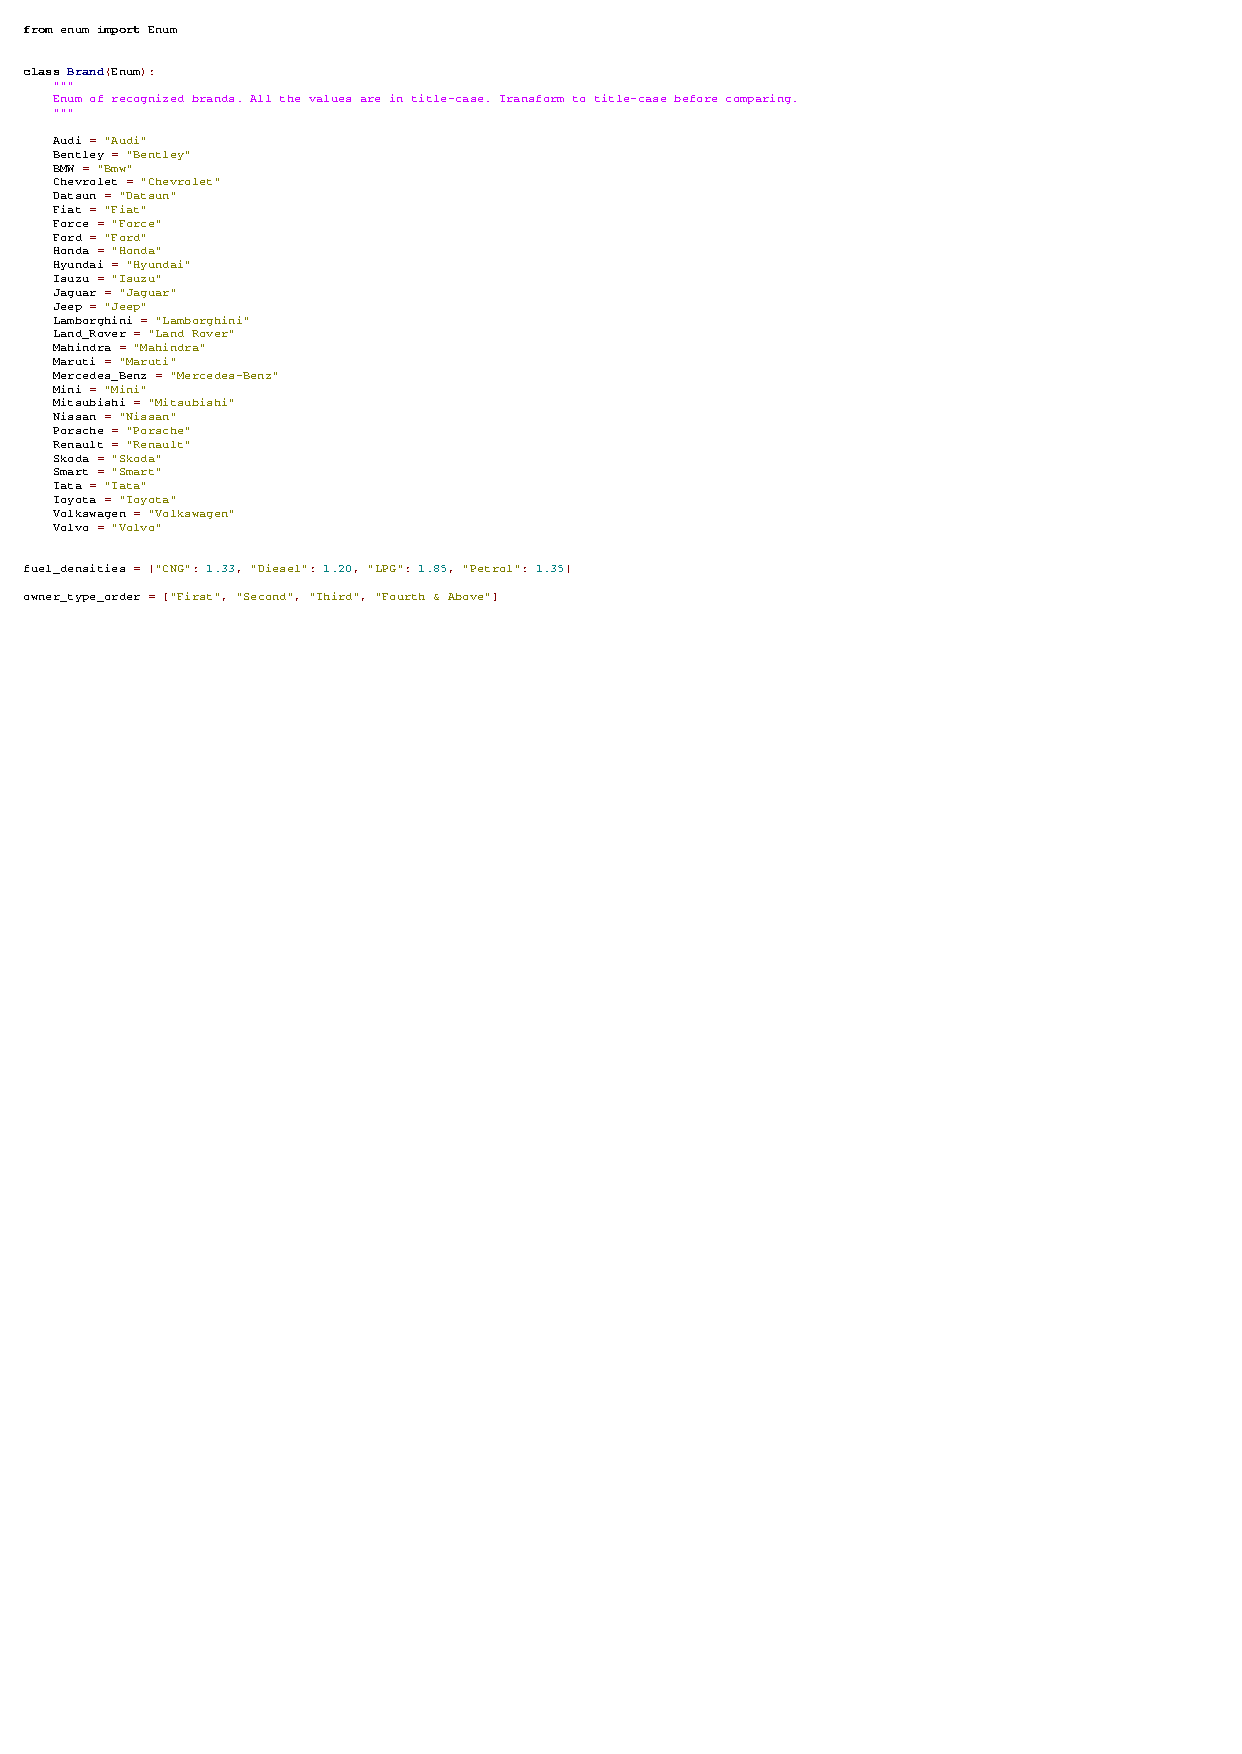
\includepdf[pages=-]{figures/codes/consts.pdf}
}


\end{document}